% !TeX spellcheck = es_ES
%----------------------------------------------------------------------------------------
%	PACKAGES AND OTHER DOCUMENT CONFIGURATIONS
%----------------------------------------------------------------------------------------

\documentclass[fleqn,10pt]{SelfArx} % Document font size and equations flushed left
%\usepackage{chemmacros}
\usepackage{ifthen}
\usepackage{calc}
\usepackage{microtype}
\usepackage{ifpdf}
\usepackage[utf8]{inputenc}
\usepackage{amsmath, amsfonts, amssymb}
\usepackage{graphicx, xcolor}
\usepackage{booktabs}
\usepackage{fancyhdr}
\usepackage{lastpage}
\usepackage{titlesec}
\usepackage{titletoc}
\usepackage{enumitem}
%\usepackage{cuted}
\usepackage[version=3]{mhchem}
\usepackage{lipsum}
\usepackage{graphbox}
\usepackage{tabularx}
%----------------------------------------------------------------------------------------
%	COLUMNS
%----------------------------------------------------------------------------------------

\setlength{\columnsep}{0.55cm} % Distance between the two columns of text
\setlength{\fboxrule}{1pt} % Width of the border around the abstract

%----------------------------------------------------------------------------------------
%	COLORS
%----------------------------------------------------------------------------------------

\definecolor{color1}{RGB}{0,94,157} % Color of the article title and sections
\definecolor{color2}{RGB}{255,243,210} % Color of the boxes behind the abstract and headings

%----------------------------------------------------------------------------------------
%	HYPERLINKS
%----------------------------------------------------------------------------------------

\usepackage{hyperref} % Required for hyperlinks
\hypersetup{hidelinks,colorlinks,breaklinks=true,urlcolor=color2,citecolor=color1,linkcolor=color1,bookmarksopen=false,pdftitle={Title},pdfauthor={Author}}

%----------------------------------------------------------------------------------------
%	ARTICLE INFORMATION
%----------------------------------------------------------------------------------------

\JournalInfo{L. de Qu\'imica inorg\'anica II, No. 4, 2016-20} % Journal information
%\Archive{Additional note} % Additional notes (e.g. copyright, DOI, review/research article)

\PaperTitle{Comportamiento Magn\'etico} % Article title

\Authors{Juan Barbosa{\color{color1}\textsuperscript{1}\textsuperscript{,2}*},
	Alejandro Camacho{\color{color1}\textsuperscript{1}\textsuperscript{,3}**}} %
%Authors
\affiliation{{\color{color1}\textsuperscript{1}}\textit{Departamento de Qu\'imica, Universidad de los Andes, Bogot\'a, Colombia}} % Author affiliation
\affiliation{{\color{color1}\textsuperscript{2}}\textit{Departamento de F\'isica, Universidad de los Andes, Bogot\'a, Colombia}} % Author affiliation
\affiliation{{\color{color1}\textsuperscript{3}}\textit{Departamento de	F\'isica, Universidad Nacional, Bogot\'a, Colombia}}
\affiliation{{\color{color1}*}\textbf{Email}: js.barbosa10@uniandes.edu.co} %
%Corresponding author
\affiliation{{\color{color1}**}\textbf{Email}: a.camacho10@uniandes.edu.co}
\Keywords{susceptibilidad magnética, balanza de Gouy, configuración electrónica, compuesto de coordinación, estado de oxidación.} %
%Keywords - if you don't want any simply remove all the text between the curly
%brackets
\newcommand{\keywordname}{Keywords} % Defines the keywords heading name

%----------------------------------------------------------------------------------------
%	ABSTRACT
%----------------------------------------------------------------------------------------
\Abstract
{
Tras sintetizar algunos compuestos y comparar su  comportamiento magnético se entiende la importancia de la medida realizada debido a a la gran cantidad de información que proporciona acerca de la naturaleza de un complejo sus enlaces, sus propiedades y posibles aplicaciones. Además dada la sencillez  de los instrumentos utilizados la medida aunque resulto ser inexacta, se puede mejorar con mucha facilidad, cambiando la estructura del montaje agregando otro imán como se muestra en el gráfico provocando que el campo aplicado sea en su mayor parte perpendicular al compuesto y no se pierda en tensiones difíciles de medir y la practica del experimentador y el numero de puntos en la curva de calibración para que se repita la medida con menor error sistemático asociado.
}
%----------------------------------------------------------------------------------------

\begin{document}
	\flushbottom % Makes all text pages the same height
	\maketitle % Print the title and abstract box
	%\tableofcontents % Print the contents section
	\thispagestyle{empty} % Removes page numbering from the first page
	%----------------------------------------------------------------------------------------
	%	ARTICLE CONTENTS
	%----------------------------------------------------------------------------------------
	\section*{Introducci\'on}
	El estudio de las propiedades magnéticas de los cuerpos ha atraído a los hombres desde la edad antigua sin embargo solo hasta llegado el tiempo de Faraday y hasta identificarse que todas la sustancias poseían propiedades magnéticas no se comenzó el estudio riguroso, que hoy combinado con el desarrollo de la física y la química es una de las propiedades de mayor potencia a la hora de identificar y caracterizar nuevos materiales y sus propiedades. 
	La medida la susceptibilidad magnética de una sustancia da cuenta de la distribución electrónica en los niveles  de energía, la configuración (bajo o alto spin), la fuerza o naturaleza de enlaces en el compuesto de coordinación, la conductividad eléctrica, la conductividad térmica e incluso la densidad de la sustancia.
	Esta propiedad se puede medir en principio con la balanza de Gouy, que es hoy día un instrumento de interés didáctico e histórico aunque resalta por su capacidad de obtener información con medios bastante limitados y sencillos la balanza de Gouy como se muestra en \autoref{fig: Gouy}, consta de una balanza en la que se han acoplados imanes que en caso de interactuar con la muestra alteran el equilibrio de la misma con posibilidad de cuantificar la fuerza o el peso de diferencia y con esto la interacción entre el compuesto y el campo, que mas tarde con las aproximaciones y consideraciones del caso permiten calcular la susceptibilidad magnética del compuesto, la cantidad de electrones desapareados, la configuración del compuesto, las propiedades de los ligandos, la geometría del compuesto, entre otras propiedades, permitiendo en cierta forma dados otras medidas o tendencias similares, describir propiedades del material o compuesto estudiado caracterizándolos para su futura aplicación.
	
	En particular medidas exactas de la susceptibilidad magnética son necesarias en el estudio de compuestos complejos dado que la misma versatilidad en los estados de oxidación de los metales de transición que abre diferentes fronteras en aplicaciones como medicina catálisis y nanotecnología y hacen interesante y necesario su estudio, dificulta  la identificación y la medida de las características dependientes del efecto del campo en el compuesto.
	
	\begin{figure}[h]
        \centering
        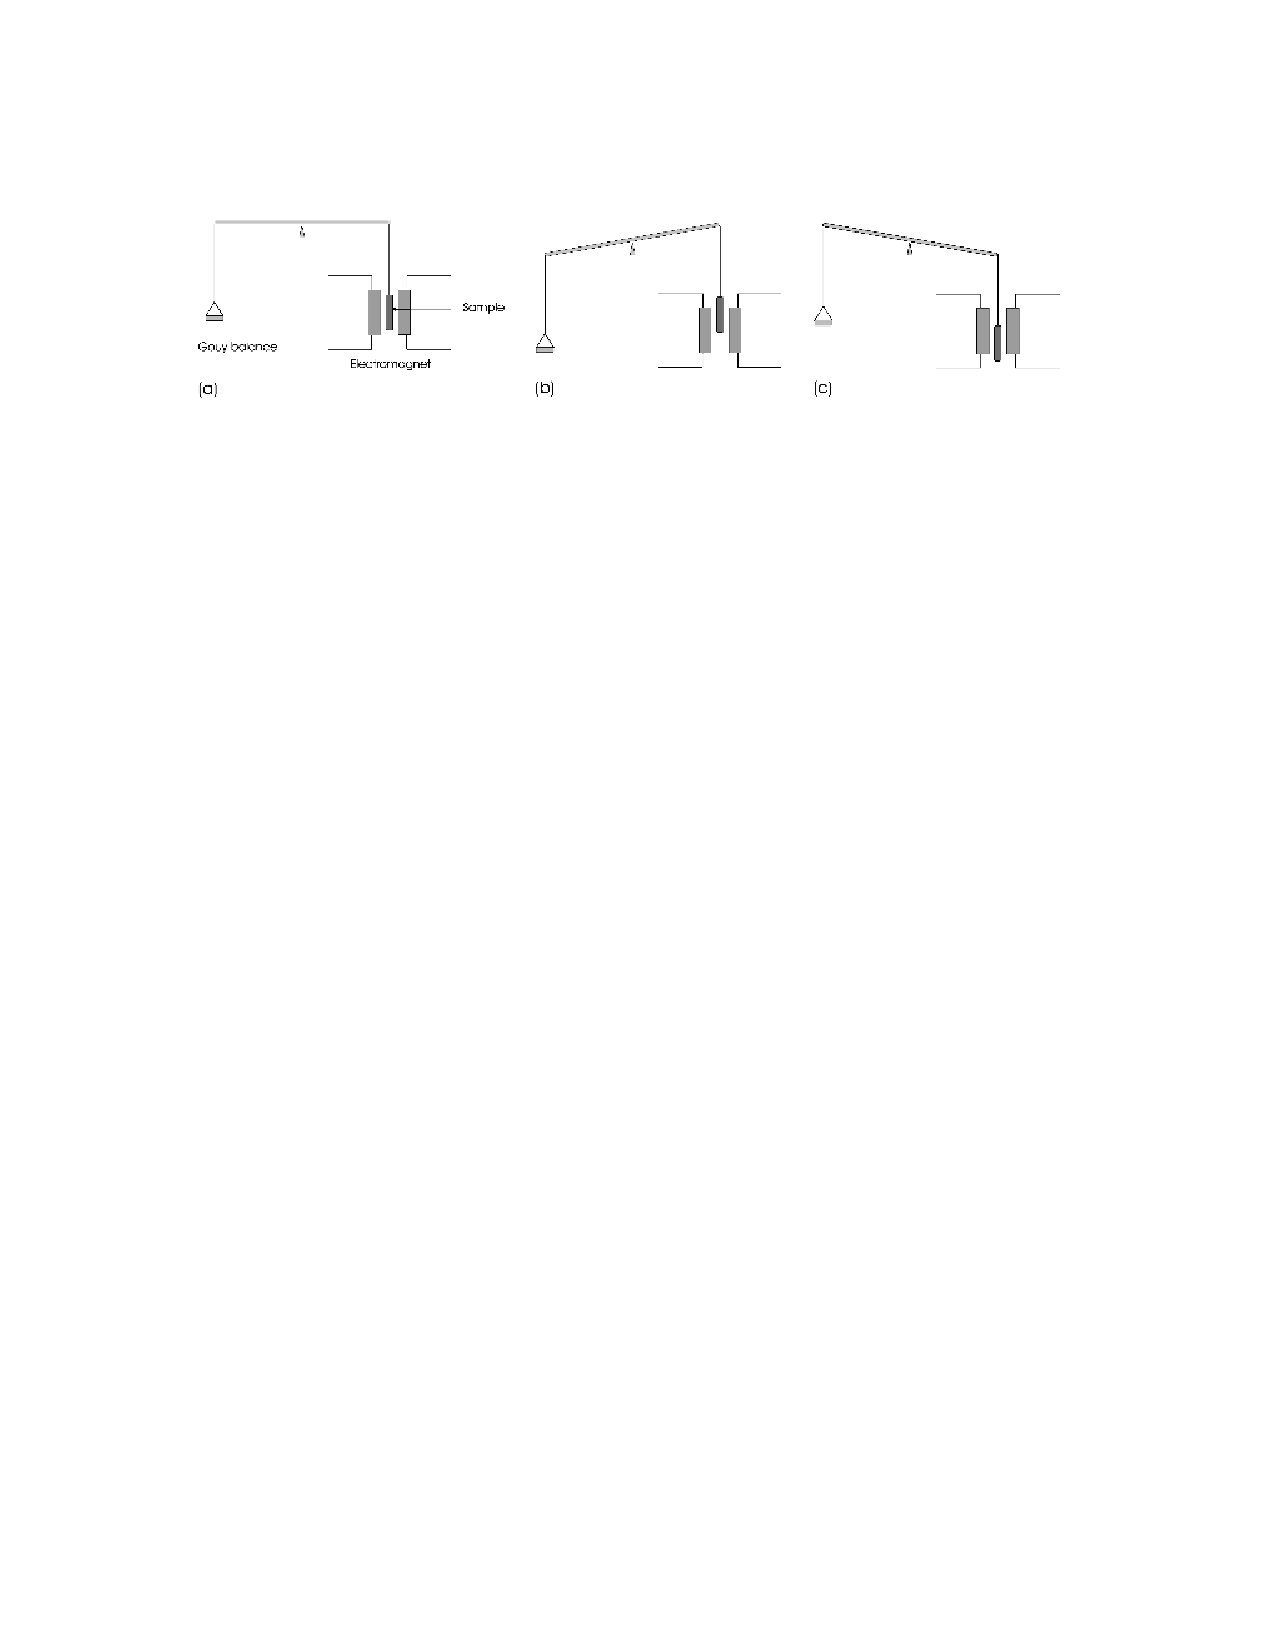
\includegraphics[width=\linewidth]{images/Gouy_balance.pdf}
        \caption{Balanza de Gouy.  (a) en ausencia de campo magn\'etico. (b) material diamagn\'etico. (c) material paramagn\'etico \cite{Materials}.}
        \label{fig: Gouy}
    \end{figure}
    
	\section{Metodolog\'ia}
	Se sintetizaron dos compuestos para el estudio de su comportamiento magnetico, a saber: El acetato de cobre monohidratado $\ce{2[Cu(OOCCH_{2})_{2}]\cdotH_{2}O}$ y el tris(2,4-pentadionato)cromo(III) $\ce{[Cr(acac)_{3}]}$. Para la síntesis del acetado de cobre monohidratado se disolvieron 0,8 g de $\ce{(CuSO_{4})\cdot 5H_{2}O}$ en 25 mL de agua y se calentó entre 50 y 60 $\ce{\circ}$ C. Luego se adicionó amoniaco al 30\% a la solución caliente con permanente agitación hasta que la solución se torno azul intensa, se agrego NaOH y se precipito el $\ce{Cu(OH)_{2}}$. Después de filtrar y lavar el solido con tres porciones de agua destilada tibia de 2 mL cada una el compuesto se disolvió en ácido acético al 10\% y se calentó en el baño de arena hasta estar próxima la sequedad, se filtro y se puso en el desecador. Para el calculo y la medida posterior. 
	
	Ahora para la síntesis del tris(2,4-pentadionato)cromo(III) a falta de (2,4-pentadiona) se utilizo (1,4-pentadiona) lo que altero las características del compuesto obtenido sin embargo el proceso de preparación fue el siguiente: Se tomaron 1,3 g de  $\ce{CoCl_{3} \cdot 6(H_{2}O)}$ y se disolvieron en 20 mL de agua donde posteriormente se agregaron 5 gramos de Urea y 4 mL de de la (q,4-pentadiona). Se calento durante una ahora a reflujo y se obtuvo un compuesto marrón claro pero no se obtuvo el precipitado café rojizo esperado, por lo que se asume el ligando un poco mas amplio en la distancia de sus dientes no logra quelar el metal por la tensión adicional que esto representa o que dado el sistema no conjugado no se presenta la estabilidad necesaria para que el compuesto actue como un ligando bidentado.
	Posteriormente los copmpuesto obtenidos en otras practicas son analizados usando la balanza de gouy para determinar la susceptibilidad magnética de los mismos.
	

	\section{Resultados y Discusi\'on}
	La s\'intesis del acetato de cobre (II) monohidratado se puede analizar en etapas, en primer lugar con la disoluci\'on de la sal de cobre en agua se obtiene cobre (II) hexahidratado. Con la adici\'on de amoniaco se libera amoniaco y se obtiene un precipitado de hidroxido de cobre (II).
	\footnotesize
	\begin{equation}
	    \begin{array}{rcl}
	        \ce{NH3 + H2O} & \ce{<=>} & \ce{NH4+ + OH-} \\
	        \ce{[Cu(H2O)6]^{2+} + 2OH-} & \ce{<=>} & \ce{Cu(OH)2.2H2O + 2H2O} 
	    \end{array}
	\end{equation}
	\normalsize
	
	Al continuar con la adici\'on de amoniaco se alcanza la formaci\'on de \ce{[Cu(NH3)4(H2O)2]^{2+}} seg\'un la siguiente reacci\'on.
	\footnotesize
	\begin{equation}
	    \ce{[Cu(H2O)6]^{2+} + 4NH3 <=> [Cu(NH3)4(H2O)2]^{2+} + 4H2O}
	\end{equation}
	\normalsize
	
	Al agregar hidr\'oxido de sodio se obtiene hidr\'oxido de cobre (II) libre de impurezas. Posteriormente se realiza una reacci\'on \'acido base entre el hidr\'oxido y el \'acido ac\'etico.
	\begin{equation}
	    \ce{Cu(OH)2 + CH3OOH -> Cu(CH3OO)2 + H2O}
	\end{equation}
	
	En el caso del acetilacetonato de cromo (III) se genera el anion al desprotonar uno de los carbonilos con amoniaco producido \textit{in situ} por la descomposici\'on de la \'urea.
	\begin{equation}
	    \begin{array}{rcl}
	        \ce{NH2COCH2 + H2O} & \ce{->} & \ce{2NH3 + CO2} \\
	        \ce{acacH + NH3} & \ce{<=>} & \ce{acac-} + NH4 
	    \end{array}
	\end{equation}
	
	Finalmente tiene lugar la reacci\'on con el cromo.
	\begin{equation}
	    \ce{Cr(H2O)6 + 3acac- -> Cr(acac)3 + 6H2O}
	\end{equation}
	
	Lamentablemente en el laboratorio no fue posible usar acetilacetonato, y fue usado 4 oxopentanal. El producto no fue el deseado debido a que el \'ultimo carece de estructuras resonantes que le permitan actuar como un ligando bidentado, como se observa en el \autoref{sch: acac}. Por esta raz\'on se cree que el amoniaco se coordin\'o al cromo dando lugar al cloruro de hexaamincromo (III).
	\begin{scheme}
	    \centering
	    \begin{tabular}{c}
	        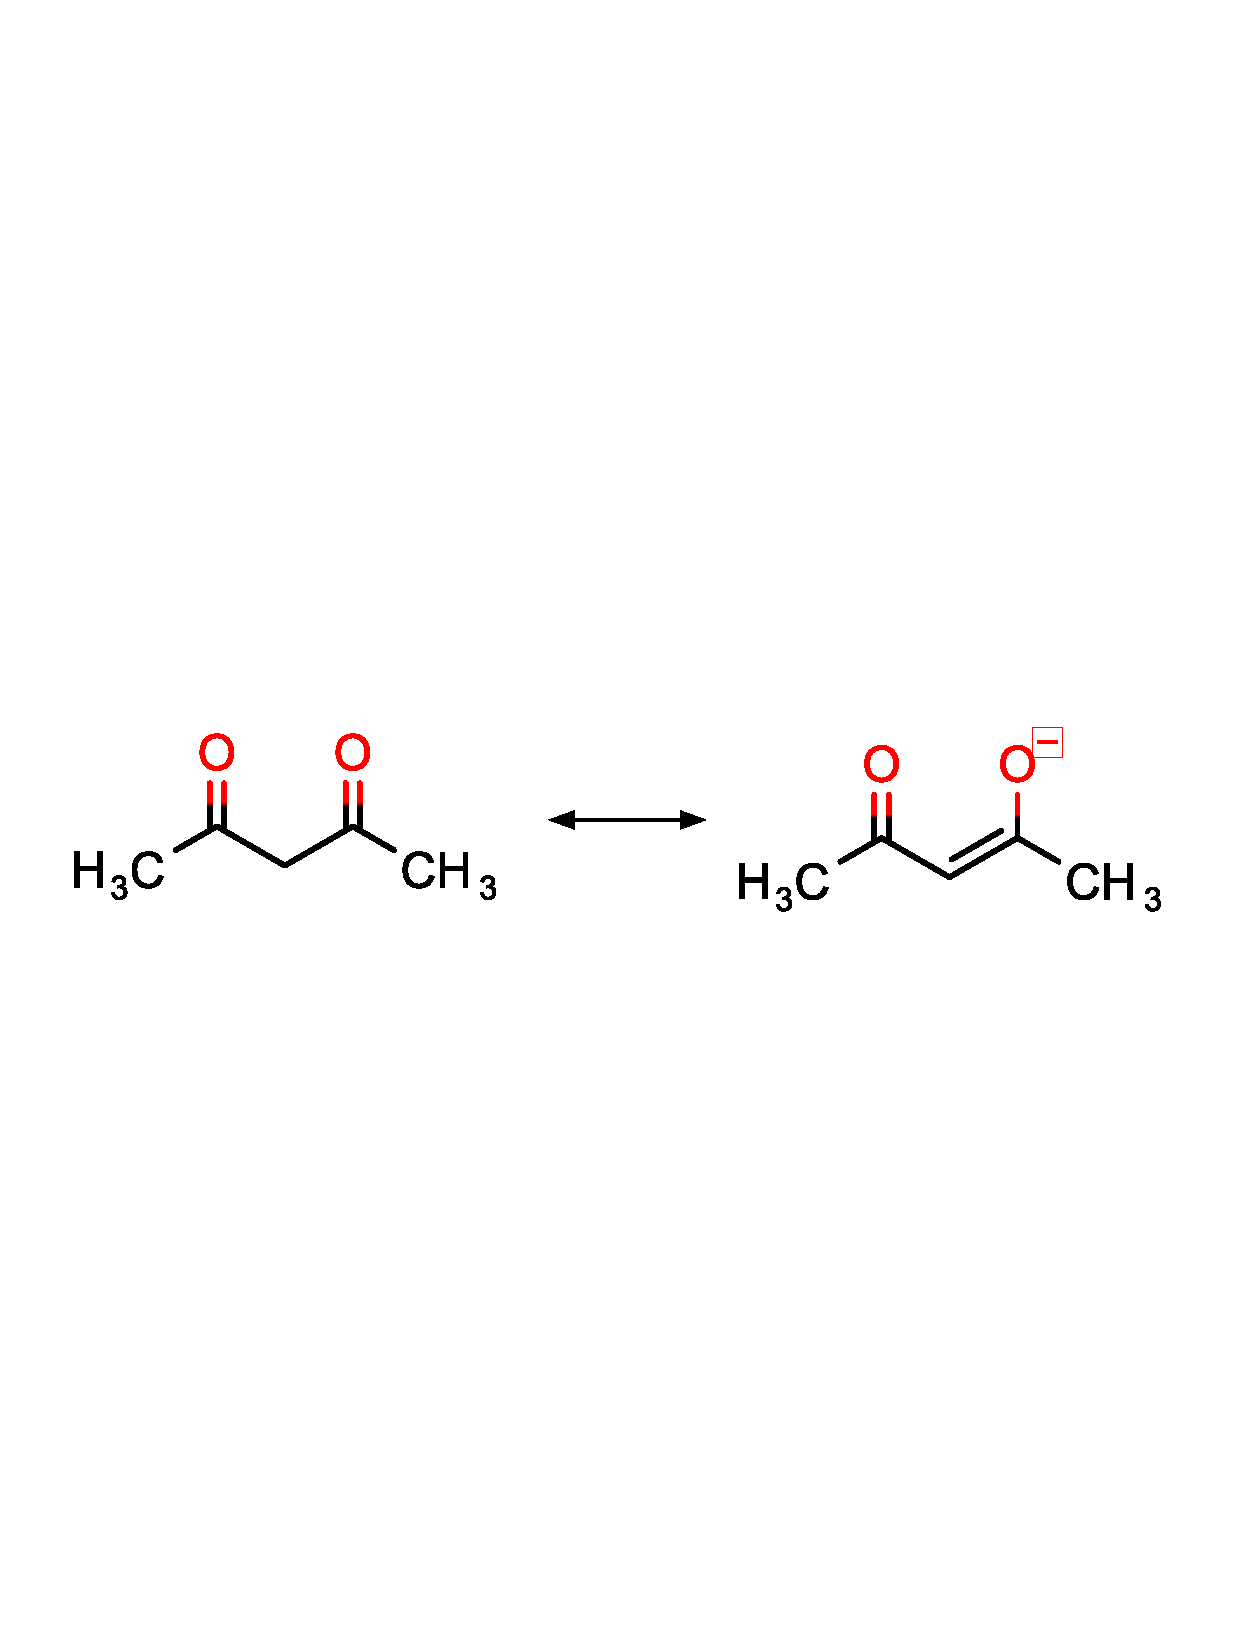
\includegraphics[width=0.9\linewidth]{images/acac.pdf}\\
	        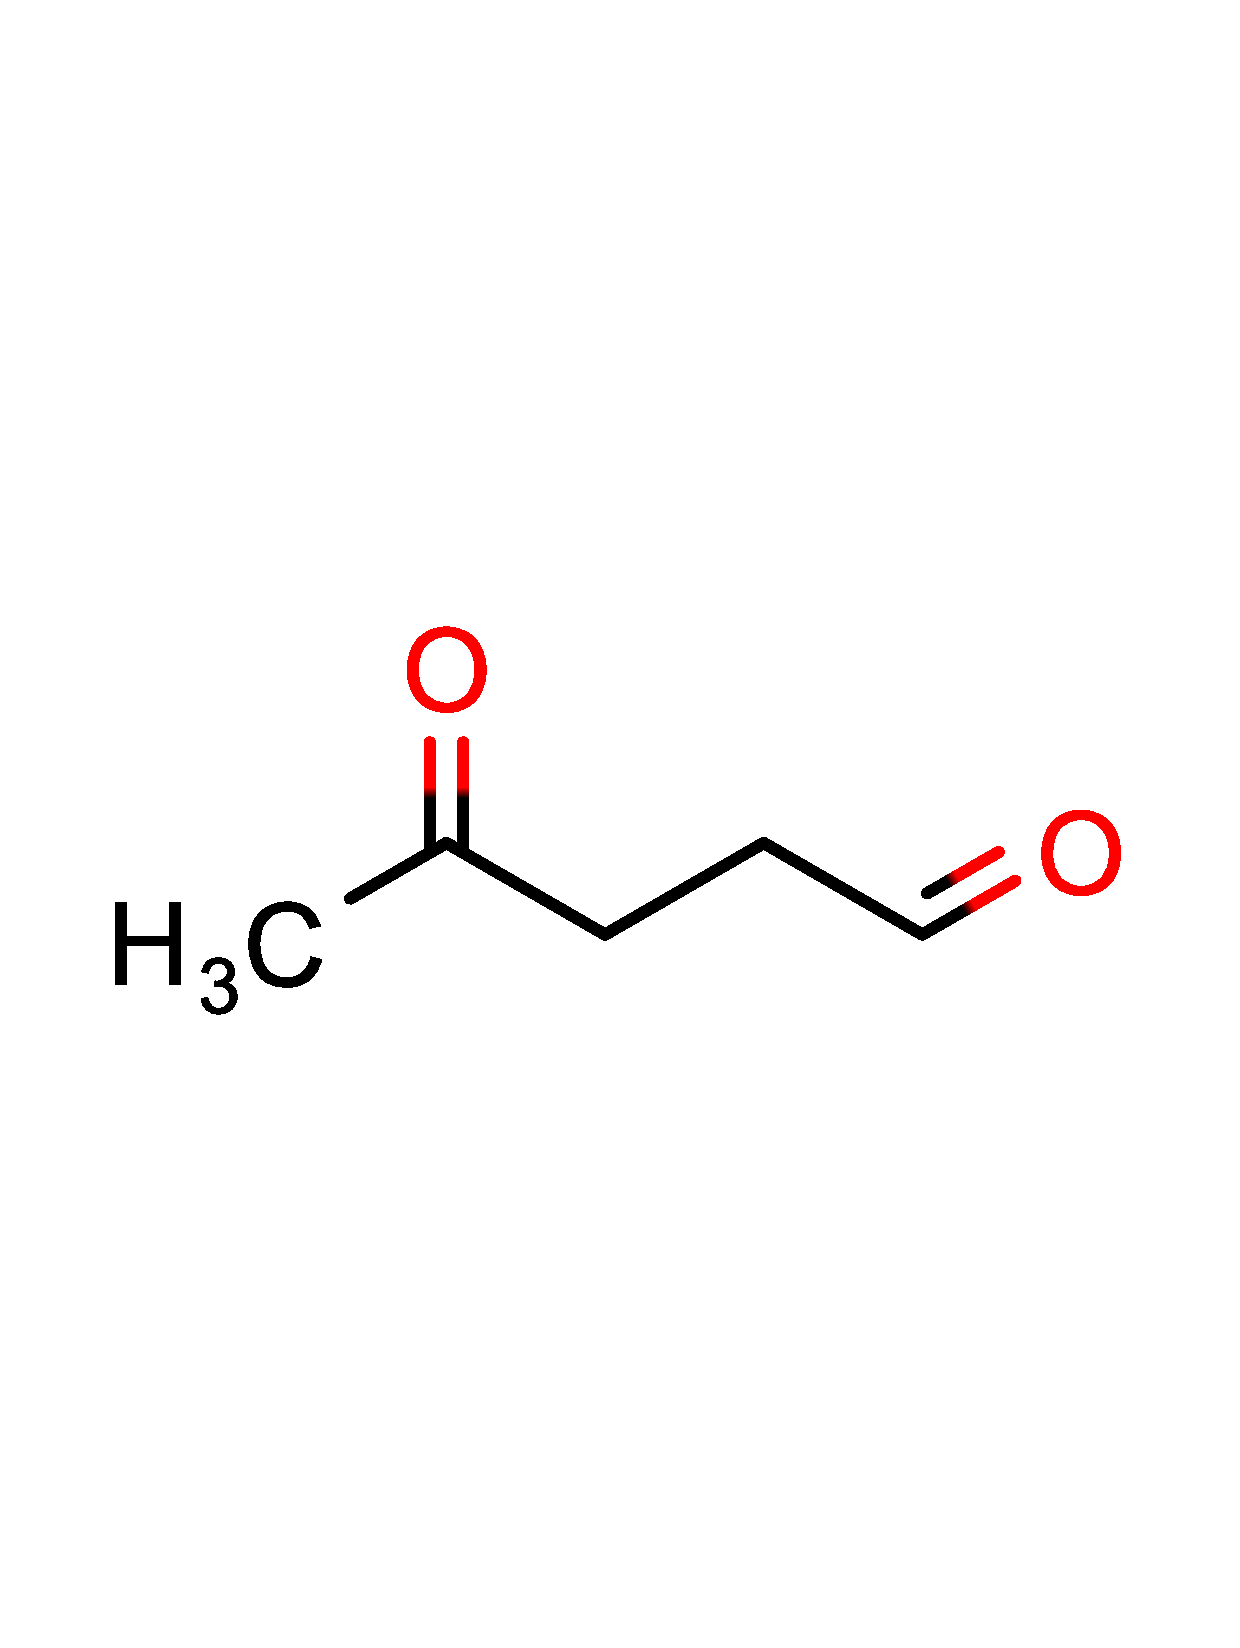
\includegraphics[width=0.4\linewidth]{images/notacac.pdf}
	    \end{tabular}
	    \caption{Estructuras resonantes estables para la 2,4 pentadiona y 4 oxopentanal.}
	    \label{sch: acac}
	\end{scheme}
	
	Por \'ultimo la reacci\'on de manganeso empieza con la reacci\'on entre el Mn (II) y acetato de sodio.
	\begin{equation}
	    \ce{MnCl2 + 2OAc -> 2HCl + Mn(OAc)2}
	\end{equation}
	
	Posteriormente tiene lugar una oxidoreducci\'on del manganeso (VII) y (II) que da lugar a la especie +3, y finalmente se obtiene el producto \ce{Mn(CH3COCHCOCH3)3}.
	\begin{equation}\label{eq: redox}
	    \begin{array}{rcl}
	        \ce{Mn^{7+} + 4e^-} & \ce{->} & \ce{Mn^{3+}}\\
	        \ce{4Mn^{2+}} & \ce{->} & \ce{4Mn^{3+} + 4e-}
	    \end{array}
	\end{equation}
	
	Para obtener informaci\'on sobre el comportamiento magn\'etico de una sustancia, lo m\'as sencillo es someterla a un campo magn\'etico y estudiar el tipo de interacci\'on. En el caso del m\'etodo experimental usado se tiene una diferencia de masas producto del campo magn\'etico generado por un im\'an.
	\begin{figure}[h]
	    \centering
	    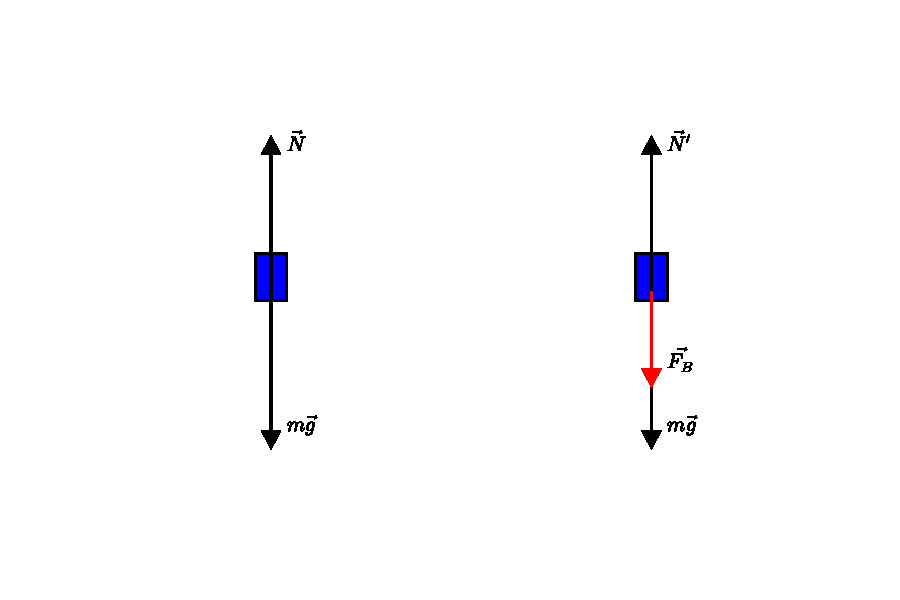
\includegraphics[width=0.7\linewidth]{images/free_body.pdf}
	    \caption{Diagrama de cuerpo libre para el montaje usado en el laboratorio.}
	    \label{fig: freebody}
	\end{figure}
	
	Usando la \autoref{fig: freebody} es posible obtener una ecuaci\'on para la fuerza producida por el campo sobre la muestra.
	\begin{equation}
	    \begin{array}{rcl}
	        N' & = & m_bg = F_b - mg \\
	        F_b & = & (m_b-m)g = - \Delta mg
	    \end{array}
	\end{equation}
	
	La ecuaci\'on anterior permite medir la magnitud de la fuerza en funci\'on de la masa registrada por una balanza. Adem\'as si se tiene en cuenta el comportamiento de materiales diamagn\'eticos y paramagn\'eticos como en la \autoref{fig: Gouy}, si $\Delta m>=0$ el material se ve repelido por el campo magn\'etico y la fuerza es hacia arriba (diamagn\'etico), lo contrario sucede con materiales paramagn\'eticos, los cuales se ven atra\'idos hacia el campo. 
	
	Los datos para la construcci\'on de la curva de calibraci\'on se muestran a continuaci\'on.
	\begin{table}[h]
	    \centering
	    \caption{Datos usados para la calibraci\'on. $\Delta m/n$ corresponde con la diferencia de masa obtenida por unidad molar en g/mol, $\chi_M$ es la susceptibilidad magnetica molar reportada en emu mol y $N$ el n\'umero de electrones desapareados}
	    \small
	    \begin{tabular}{c|ccc}
	        \hline
	        \textbf{Compuesto} & $\Delta m/n$ & $\chi_M$ & $N$ \\
	        \hline
	        FeCl$_3$ · 6H$_2$O & -10.704 & 15.250 & 5.0 \\
            MnSO$_4$ · H$_2$O & -12.494 & 14.200 & 5.0 \\
            Fe$_2$(SO$_4$)$_3$ · 9H$_2$O & -10.158 & 11.200 & 4.0 \\
            CoCl$_2$ · 6H$_2$O & -7.890 & 9.710 & 3.0 \\
            KCr(SO$_4$)$_2$ · 12H$_2$O & -3.691 & 6.200 & 3.0 \\
            NiSO$_4$ · 6H$_2$O & -7.620 & 4.300 & 2.0 \\
            CuSO$_4$ · 5H$_2$O & -1.783 & 1.570 & 1.0 \\
            Fe$_4$[Fe(CN)$_6$] & -8.710 & -172 & 0.0 \\
            (NH$_4$)$_2$Cr$_2$O$_7$ & -0.075 & 38 & 0.0 \\
            CuCl & -0.787 & -40 & 0.0 \\
            \hline
	    \end{tabular}
	    \normalsize
	    \label{tab: calibrationData}
	\end{table}
	
	En la \autoref{fig: calibrationCurves} se tienen las ecuaciones de las rectas obtenidas por m\'inimos cuadrados. Para la gr\'afica izquierda no se reporta incertidumbres dado que el rango pertenece a los n\'umeros enteros. Para la susceptibilidad se tienen incertidumbres de 0.35 emu/g para la pendiente y 3.0 emu/mol para el intercepto.
	\begin{figure*}[h]
	    \centering
	    \begin{tabular}{cc}
	        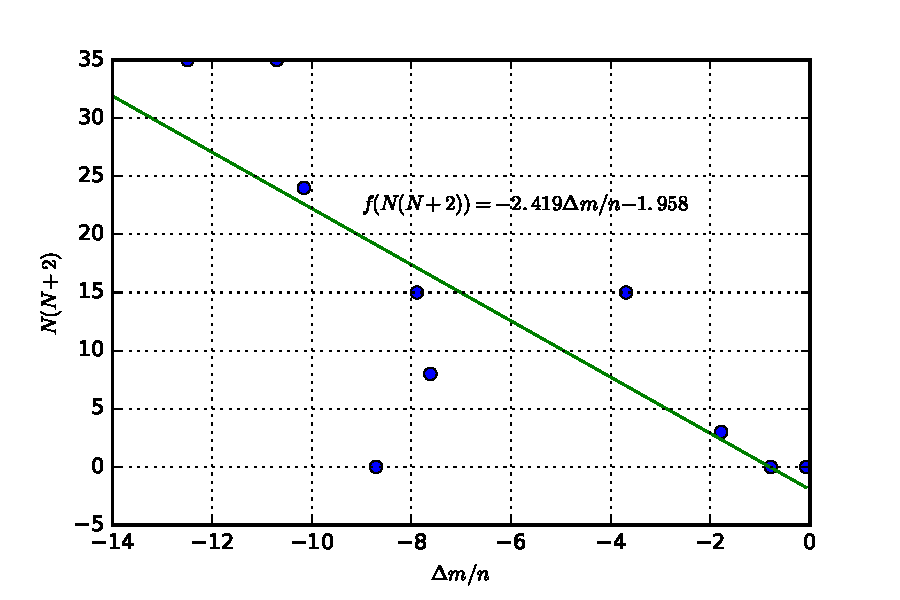
\includegraphics[width=0.5\linewidth]{images/Unpair_Mass.pdf} & 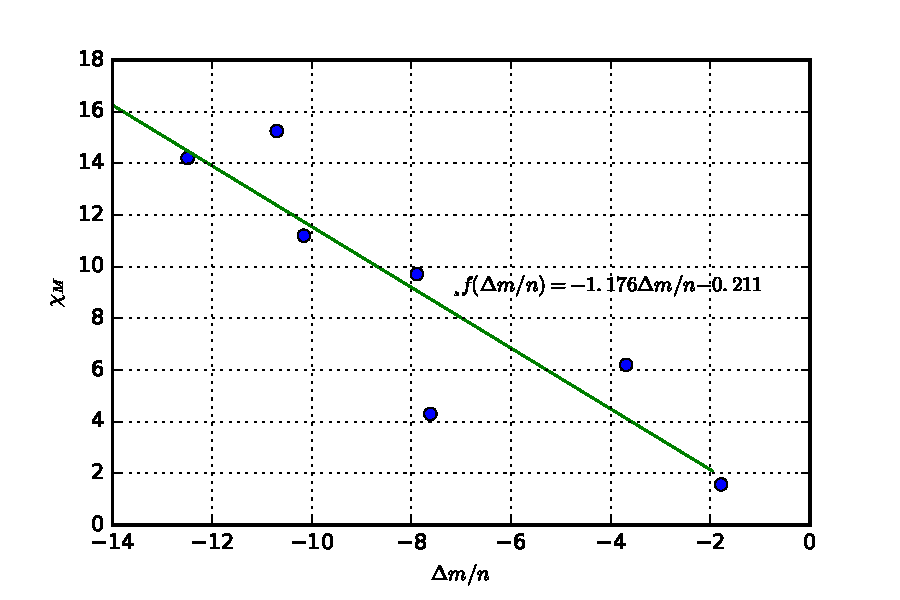
\includegraphics[width=0.5\linewidth]{images/Susceptibility_mass.pdf} \\
	    \end{tabular*}
	    \caption{Curvas de calibraci\'on para el n\'umero de electrones desapareados y la suceptibilidad magn\'etica molar.}
	    \label{fig: calibrationCurves}
	\end{figure*}
	
	Los resultados obtenidos para las muestras sintetizadas se muestran a continuaci\'on:
	\begin{table}[h]
	    \centering
	    \caption{Resultados obtenidos para los distintos compuestos sintetizados en el laboratorio. Se debe tener en cuenta que no todas las mediciones fueron realizadas el mismo d\'ia.}
	    \begin{tabular}{c|ccc}
	        \hline
	        \textbf{Compuesto} & $\Delta m/n$ & $N$ & $\chi_M$ \\
	        \hline
	        \ce{Cu2(OAc)4.H2O} & -2.314 & 0.80 & 2.511 \\
	        \ce{Cr(acac)3} & - & - & - \\
	        \ce{trans-[CoCl2(en)2]Cl} & -0.843 & 0.55 & 0.780 \\
	        \hline
	    \end{tabular}
	    \label{tab: results}
	\end{table}
	
	Para el caso del acetato de cobre monohidratado, se obtiene un electr\'on desapareado y una susceptibilidad magn\'etica de 2.511 emu mol. Lo anterior concuerda con lo esperado dado que el cobre presenta un estado de oxidaci\'on (II) por lo cual se comporta como un d$^9$. Al tener un exponente impar implica que debe tener al menos un electr\'on desapareado, sin embargo como existen solo cinco orbitales d, existe solo un electr\'on desapareado. El valor es un poco m\'as bajo debido a el enlace metal metal, este enlace ocasiona que los espines desapareados est\'en orientados en la direcci\'on opuesta y el efecto neto del campo se anule.
	
	Para el caso del tris-acetilacetonato de cromo (III) no fueron tomados datos magn\'eticos por complicaciones en su s\'intesis. En \'ultimo lugar est\'a el trans-cloruro de diclorobis (etilendiamina) cobalto(III), para \'el existen dos configuraciones posibles, una de alto sp\'in y otra de bajo sp\'in.
	\begin{figure}[h]
	    \centering
	    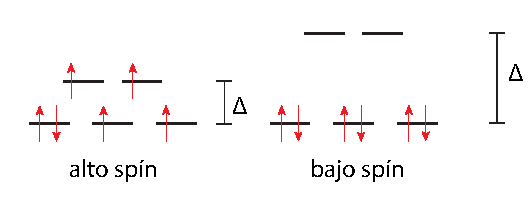
\includegraphics[width=\linewidth]{images/CoSpin.pdf}
	    \caption{Distintas configuraciones electr\'onicas para el complejo de cobalto (III).}
	    \label{fig: CobaltSplit}
	\end{figure}
	
    Con el objetivo de dar explicaci\'on a los resultados experimentales es necesario adem\'as usar la serie espectroqu\'imica para la cual se establece que el ligando en tiende a aumentar la energ\'ia del campo del ligando, de la misma forma que lo hace el cloruro en menor proporci\'on. Debido a esto las observaciones de un posible diamagnetismo coinciden con lo esperado.
	
	\section{Preguntas}
	\subsection{?`Cu\'al otra indicaci\'on f\'isica, aparte del momento magn\'etico, podr\'ia conducir a la conclusi\'on que un enlace metal-metal est\'a presente en este compuesto?}
	De existir un enlace metal-metal el complejo debe exhibir propiedades propias de los metales, como conductividad t\'ermica y el\'ectrica, los cuales se pueden medir f\'acilmente con mult\'imetros y term\'ometros.
	
	\subsection{La baja susceptibilidad magn\'etica podr\'ia ser explicado por otras razones diferentes, aunque parece indicar que un enlace metal-metal est\'a presente.}
	Como se discute en el an\'alisis el enlace metal metal tiene en cuenta los electrones desapareados de ambos n\'ucleos met\'alicos y los restringe a tener direcciones distintas de esta forma se obtiene un compuesto con un comportamiento menos paramagn\'etico de lo esperado.
	
	\subsection{Una de las clases principales de compuestos que forman enlaces metal-metal son los complejos con CO. Discuta este tipo de enlace con dos miembros de este grupo.}
	Los complejos con mon\'oxido de carbono hacen parte de la familia de los compuestos organomet\'alicos, la capacidad de formaci\'on de enlaces metal metal proviene de dos propiedades distintas. En primer lugar est\'a la capacidad $\pi$ aceptora, la interacci\'on metal ligando es una integracci\'on $\sigma$ sin embargo existe una interacci\'on $\pi$ adicional que se origina cuando los orbitales d del metal interactuan con los p del mon\'oxido de carbono, en ese sentido la mol\'ecula CO permite retrodonaci\'on estabilizando la carga del metal. Por otro lado existe la posibilidad de isomerizaci\'on de estos complejos como es el caso del octacarbonilo de dicobalto.
	\begin{figure}[h]
	    \centering
	    \begin{tabular}{c}
	        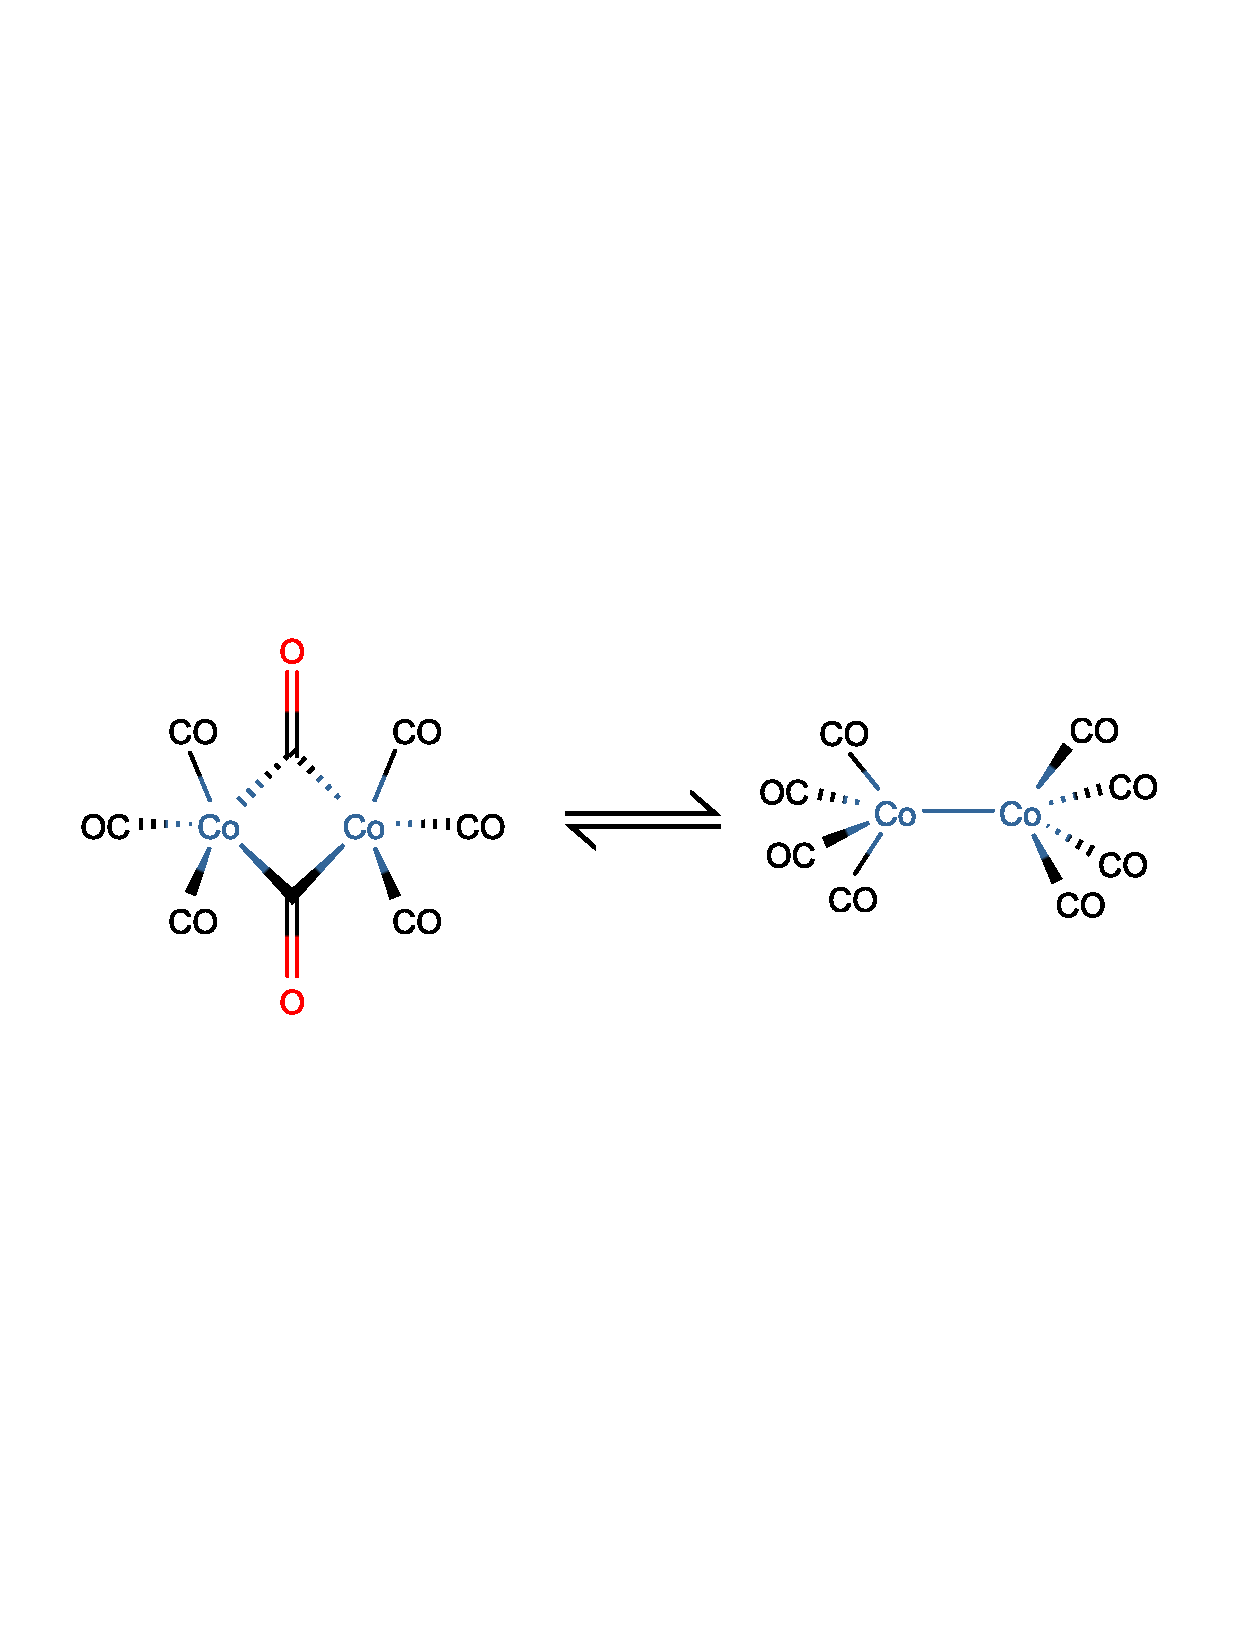
\includegraphics[width=\linewidth]{images/dicobalt.pdf} \\ 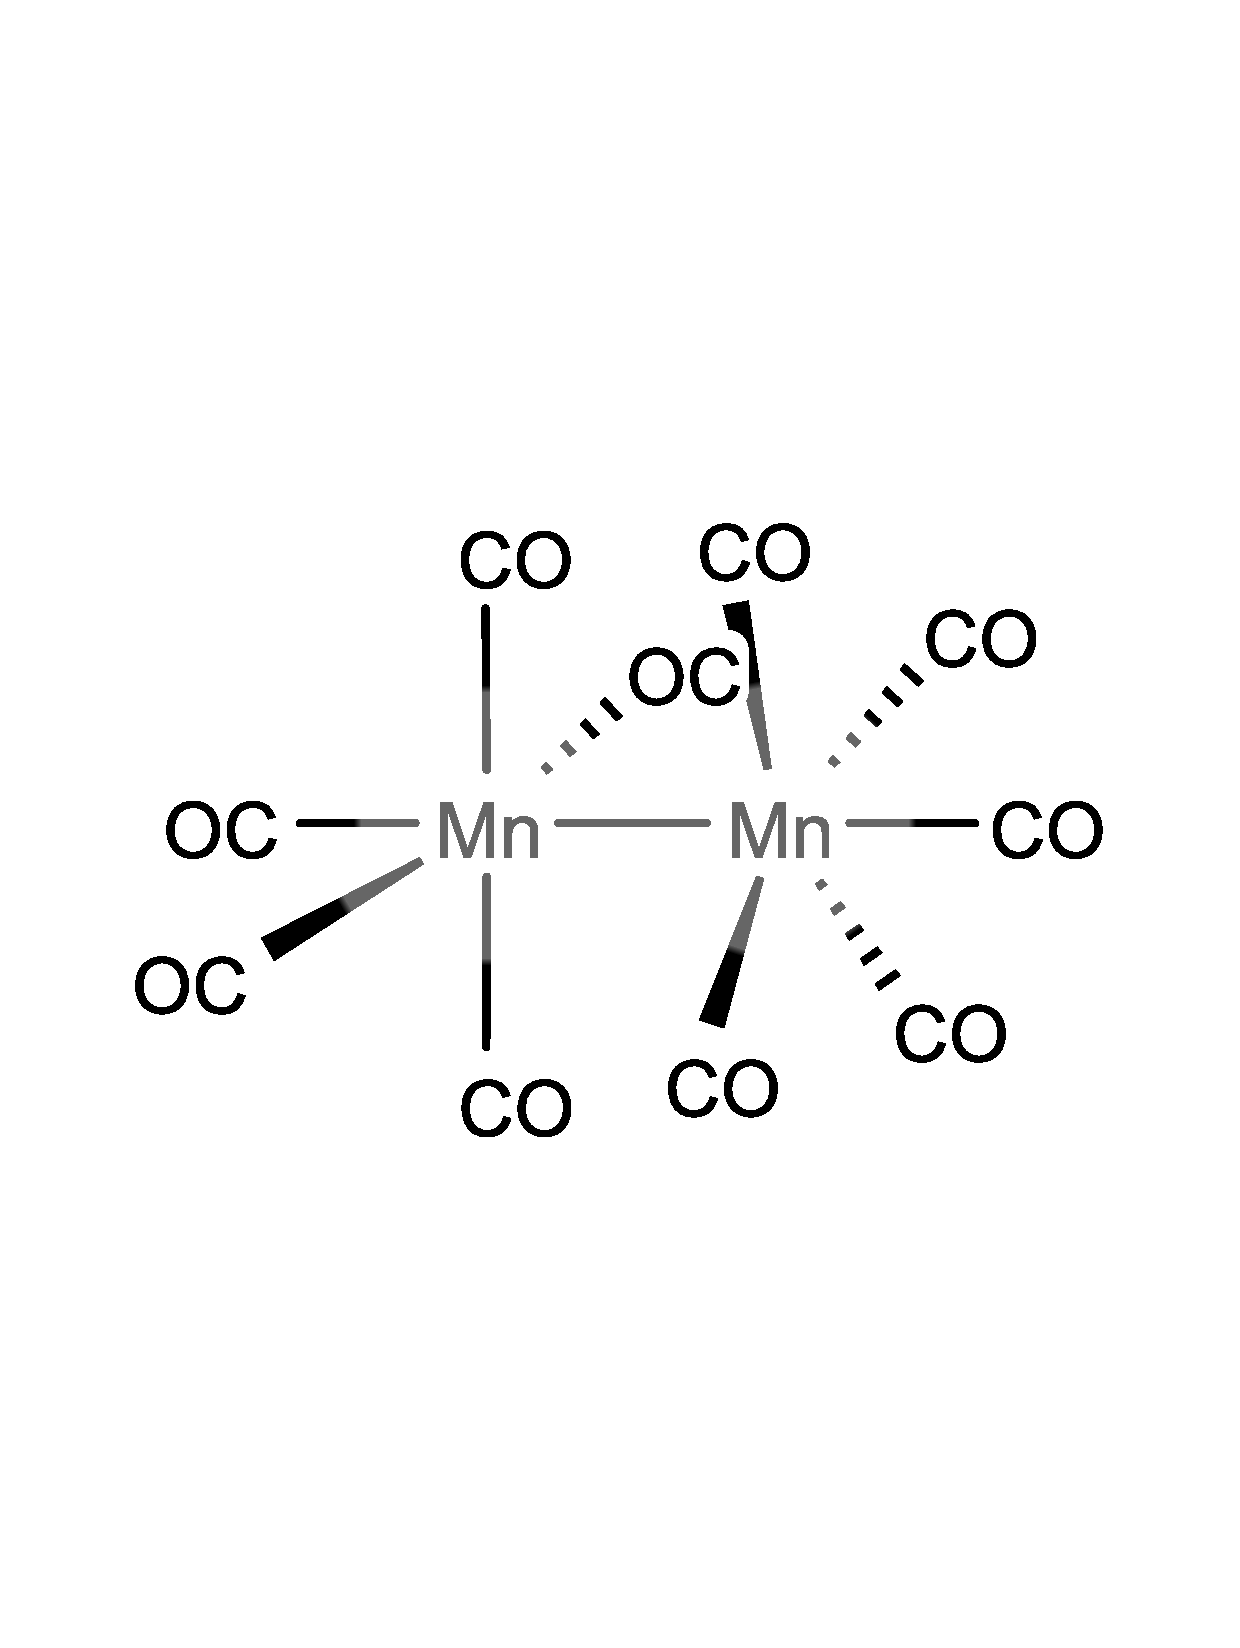
\includegraphics[width=0.5\linewidth]{images/dimanganese.pdf}
	    \end{tabular}
	    \caption{En la parte superior se muestra la isomer\'ia del \ce{Co2(CO)8}, y en la inferior el \ce{Mn2(CO)10.}}
	    \label{fig: dinucleares}
	\end{figure}
	
	\subsection{Escriba todas las reacciones redox de este experimento y balanc\'eelas}
	La reacci\'on redox involucrada en la s\'intesis del acetilacetonato de manganeso (III) se muestra en la \autoref{eq: redox}.
	
	\subsection{Cromo tiene varios estados de oxidaci\'on a parte del tres. ?`Cu\'ales son? ?`Cu\'al coloraci\'on tienen las soluciones acuosas de ellos?}
	En el cromo son comunes los estados de oxidaci\'on (VI), (III) y (II), y los colores de los complejos en soluci\'on son: amarillo/naranja, verde, y azul \cite{Nature}.
	
	\subsection{En acetona, compuestos alquinos no desprenden f\'acilmente protones tampoco en presencia de bases. En acetilacetona el prot\'on ya esta disociado formando el ani\'on acetilacetonato. ?`Por qu\'e reaccionan estos dos compuestos similares tan diferente?}
	Existen dos propiedades importantes de la acetilacetona. En primer lugar se desprotona facilmente (pKa $\approx$ 9 \cite{Harris}) lo cual da lugar a una estructura resonante bastante estable como se observa en el \autoref{sch: acac}. Por otro lado puede realizar tautomer\'ia ceto-enolica, esto es que el par electr\'onico del carbonilo forma un doble enlace entre los carbonos 2 y 3, y el hidr\'ogeno se mueve al ox\'igeno dando lugar a un alcohol.
	
	\subsection{El ion Mn(II) (d$^5$) es casi incoloro, mientras el Mn(VII) (d$^0$) es violeta oscuro. Explique}
	Para el Mn(II) de alto sp\'in todas las transiciones electr\'onicas est\'an prohibidas por paridad, por esta raz\'on el complejo no absorbe luz en el rango visible. En el caso del Mn(VII) es posible que existan transiciones electr\'onicas desde los orbitales p del nivel anterior que den lugar a la coloraci\'on observada.
	
	\subsection{Las estructuras de de \ce{Cr(acac)3} y de \ce{Mn(acac)3} son muy diferentes. ?`Cu\'al es la estructura de \ce{Mn(acac)3}?}
	La estructura del acetilacetonato de manganeso (II) es un octaedro estirado por el efecto Jahn-Teller.
	
	\subsection{?`Podr\'ian mostrar los dos compuestos \ce{Cr(acac)3} y \ce{Mn(acac)3} el efecto Jahn-Teller? Explique}
	En el caso del cromo (III) se obtiene un d$^3$ donde los tres electrones ocupan los orbitales d$_{z^2}$, d$_{xz}$, d$_{xy}$ que son los de menor energ\'ia, por esta raz\'on no exhibe efecto Jahn-Teller. Por el otro lado el complejo de manganeso se comporta como un d$^4$, existe un efecto fuerte debido a la interacci\'on del electr\'on desapareado en el orbital d$_{x^2-y^2}$ \cite{Jahn-Teller}.
	
	\section{Conclusiones}
	Las propiedades magn\'eticas de los complejos de coordinaci\'on entregan informaci\'on de vital importancia para el entendimiento de la configuraci\'on electr\'onica de los complejos y la geometr\'ia de coordinaci\'on. Adicionalmente su estudio no requiere instrumentaci\'on compleja o avanzada, por lo cual no es una t\'ecnica que requiera costos adicionales.

	\phantomsection
	\bibliographystyle{unsrt}
	\begin{thebibliography}{9}
	    \bibitem{Materials}
	    Tilley, R. J. D. \textit{Understanding solids: The science of materials}; John Wiley & Sons: Chichester, United Kingdom, 2004; pp 363–391.
	    \bibitem{Nature}
	    Lennartson, A. The colours of chromium. \textit{Nature Chemistry}. DOI: 10.1038/nchem.2068. Published Online: Sept 22, 2014, \textit{6} (10), 942–942.
	    \bibitem{Harris}
	    Harris, D. C. \textit{Quantitative chemical analysis}, 8th ed.; Freeman, W. H. & Company: New York, 2010.
	    \bibitem{Jahn-Teller}
	    Miessler, G. L.; Fischer, P. J.; Tarr, D. A. \textit{Inorganic chemistry}, 5th ed.; Prentice Hall: Boston, MA, United States, 2013; p 371.
	\end{thebibliography}
\end{document}
